\documentclass[output=paper]{langsci/langscibook} 
\author{Isabel Tejada-Sánchez\affiliation{Universidad de los Andes}\lastand Carmen Pérez-Vidal\affiliation{Universitat Pompeu Fabra} }
\title{Writing performance and time of exposure in EFL immersion learners: analysing complexity, accuracy, and fluency}
\shorttitlerunninghead{Writing performance \& time of exposure in EFL immersion learners}
 
 
\abstract{The present study explores the effects of two types of early-partial immersion programmes on writing performance in English as a Foreign Language (EFL). It examines adolescent learners (ages 12-17) in mainstream education in Colombia. The two programmes are similar as far as the learners’ onset age (4) is concerned, but different with respect to the total amount of EFL exposure time and intensity: High Intensity plus (HI+) has a total of 8,760 accumulated hours by age 17, while High Intensity (HI) has a total of 7,002 hours. It has been prevalently hypothesized that the more time students dedicate to learning the L2, the higher their level of proficiency will be (\citealt{Carroll1962,Stern1985}), supporting the spread of instructed immersion and intensive programmes \citep{SerranoEtAl2011,Lightbown2012}. One of the aims of this chapter is to further assess this hypothesis.  The study examines a cross-sectional sample (N=188), adopting a between-groups design whereby programmes’ performance is compared in terms of the effect of accumulated time. Analysis will focus on the domains of syntactic and lexical complexity, accuracy, fluency  (CAF) \citep{HousenEtAl2012} and on holistic ratings. Results indicate that learners’ writing in HI+ and HI do not show to be significantly different in most domains of CAF examined, nor in the holistic ratings. This might be explained in the light of the prior high number of accumulated hours of English exposure and emphasis on literacy in the curriculum of both programmes, which has allowed learners to reach a threshold level from which they do not regress (\citealt{Bournot-Trites2007,Williams2012}).}
\maketitle

\begin{document}  


\section{Introduction}

Since the emergence of \isi{immersion} programmes in Canada in the late 1960s (\citealt{LambertTucker1972}), much research has been carried out on the development of \isi{linguistic} competence in an \isi{L2} in such settings (\citealt{GeneseeStanley1976,Genesee1978,Swain2000french}). The majority of these studies, mostly in favour of \isi{immersion}, have also addressed the limitations of \isi{immersion} programmes, particularly in terms of the \isi{L2} competence attained and the risks involved in the development of the L1 (\citealt{Genesee1978,Genesee2013,Lazaruk2007}). Despite these concerns, the \isi{immersion} education model has developed rapidly, inspiring bi- and \isi{multilingual} school programmes throughout the world (\citealt{DeMejia2002}). The acknowledged success of \isi{immersion} programmes may be due to a combination of factors that have been shown to positively affect \isi{L2} \isi{acquisition}, such as onset age, the type of input made available and its quantity, that is, the amount of time allocated to \isi{L2} exposure, methodological flexibility (early, middle and late programmes) and teachers’ backgrounds, among others (\citealt{Genesee2013,JohnsonSwain1997,Lazaruk2007}). 

This chapter is part of a larger study Tejada-Sanchez \citeyear{Tejada-Sanchez2014} which examines  the outcomes of \isi{immersion} programmes in Colombia, focusing on \isi{EFL} writing of L1-\ili{Spanish} speakers. More specifically, it seeks to understand the relationship between the allocation of time in the programme and the resulting learners’ written performance in their \isi{target language}, \ili{English}. This relationship has not been sufficiently addressed in studies on school \isi{immersion} contexts outside Canada, and even less so in the Colombian context. Earlier studies and compilations have underscored the importance of addressing the effect of the time factor, and more specifically intensive exposure experiences, within \isi{L2} instructional settings \citep{Muñoz2012}.  Consequently, there remains a gap in the literature as to how language productive abilities benefit from such intensive instructional experiences. Undoubtedly, the number of uncontrollable variables within educational settings, such as individual differences, curriculum and context specifics, make this a particularly complex endeavour. For this study, data collection was conducted during class time in order to ensure the students’ participation. It included written data and a background questionnaire which was used to control for individual variables such as age, \isi{L2} exposure and \isi{target language} contact hours outside the school.     

The chapter thus presents a descriptive study that evaluates the relative effect of different amounts of exposure to L2-\ili{English} in two early partial \isi{immersion} programmes in Colombia. We begin by reviewing the literature concerning time as an essential factor within \isi{immersion} programmes, to then go on to discuss writing development in terms of the \isi{CAF} triad, as well as the measurements adopted for profiling these dimensions. We then move on to present the methodology. Finally, results and analysis are outlined, followed by a discussion. Concluding remarks will focus on the implications of this study for \isi{L2} education and specifically curriculum allocation of languages within \isi{immersion} programmes in non-\ili{English} speaking contexts.

\section{Literature review}

\subsection{Time as an intrinsic factor for immersion programmes}

The question of the influence of the amount of target \isi{language exposure} on language \isi{proficiency} was raised quite early in the implementation of French \isi{immersion} programmes in Canada. Carroll’s contributions in the mid-sixties and seventies around the characteristics of \isi{immersion} programmes were fundamental. Regarding the time-skill relationship, he asserted: “There are many factors which contribute directly to the effectiveness of French instructional programs (...) Organizationally, it is considered \textit{that the key factor is the number of hours of instruction} in French (…) In other words, \textit{the more hours a pupil spends in French, the higher level of achievement is likely to be}” (\citet[8]{Carroll1975}, cited in \citet[1-2]{Swain1981}: emphasis added). He identified a direct link between the volume of input made available to learners, quantified as time, and the overall \isi{L2} attainment. \citet{Stern1985}, in turn, referred to a threshold regarding the number of hours likely to ensure a \textit{bilingual} competence in an \isi{immersion} context: at least 5,000 hours, but this account did not determine the characteristics of the learner involved in the programme, and did not make explicit the distribution of exposure time or its intensity, in terms of hours per week/month. Currently, the publications which explore time as a factor in the development of an \isi{L2} emphasize its importance but at the same time its intricate complexity.  The conclusions that can be drawn from \citegen{Muñoz2012} compilation demonstrate that, depending on how and where time is operationalized in language education, it can lead to a myriad of effects, from cognitive to socio-\isi{pragmatic}, from global language features to discrete ones such as those addressed by the \isi{CAF} dimensions. In this study, we focus on the parameter of accumulated time of exposure. This parameter refers to the global amount of time, in terms of number of hours, dedicated to \isi{L2} learning (\citealt{Stern1985,Genesee1978,Genesee2013}). It is usually required for the completion of a programme with a given target \isi{proficiency} level, as defined for instance by the CEFR descriptors (\citealt{CouncilofEurope2001}).  Regarding the accumulated time of exposure, \isi{immersion} programmes are those where L2-contact time, along with content integrated instruction, is deemed essential for the programme’s functioning (\citealt{CollinsEtAl1999}). Globally, \isi{immersion} programmes have been traditionally described as beneficial for receptive skills (\citealt{DayShapson1988}), while their limitations regarding writing and accuracy have been frequently reported in previous research (\citealt{Lightbown2012,GermainEtAl2004}). In such respect, in written and oral expression, \isi{immersion} learners often demonstrate a considerable influence of L1 grammar. Also, it has been repeatedly reported that learners would not start a conversation in the \isi{L2} spontaneously, unless when they are asked to do so (\citealt{Harley1992,Wesche2002}). Finally, it is suggested that even though productive skills appear to be distant from those of native speakers, learners in \isi{immersion} programmes continue to make progress in the \isi{L2} (\citealt{Harley1992,Wesche1989,Housen2012}).

Particularly in terms of writing, the main topic in this study, contributions by Bournot-\citet{Bournot-Trites2007}, \citet{CollinsWhite2011},\citet{TurnbullEtAl1998} and \citet{Lightbown2012} underscore learners’ capability to communicate effectively but failing to reach native-like levels, for instance as regards lexical diversity and structural elaboration.  

Summing up, it has been prevalently hypothesized that the more time students dedicate to learning the \isi{L2}, the higher their level of \isi{proficiency} will be \citep{Stern1985}, thus supporting the spread of instructed \isi{immersion} and intensive programmes (\citealt{SerranoEtAl2011,Lightbown2012}). However, although the pioneer Canadian initiatives have been abundantly documented in the \isi{SLA} literature, research is scarce as far as other countries are concerned. Hence, the current study seeks to shed light on the effects of \isi{EFL} \isi{immersion} in Colombia, by examining and comparing the effects on \isi{writing performance} of students belonging to two programmes which differ in total number of hours and their distribution. Individual differences such as \isi{L2} exposure outside school, family bilingualism, and total amount of time in the school were also taken into consideration, but will not be discussed in this chapter.

\subsection{L2 Written performance}
\largerpage
Writing is a cognitively complex and multidimensional endeavour involving different stages and processes (\citealt{Manchón2013,Ortega2012}). In fact, this skill is understood as an 'interactive' process where various factors, such as genre awareness (stylistic organization and textual format) and mastery of content and language, are frequently activated and deactivated, according to writing pace and the needs of the composition process.

Creating a text comprises three main stages, namely, planning, formulation and revision \citep{Manchón2009,Manchón2013,SilvaMatsuda2005}. In the case of an \isi{L2}, this activity is complicated by additional demands such as the search for the appropriate lexicon, grammar, discourse and other peculiar dimensions of the \isi{target language} and culture \citep{Manchón2009}. 

In this study, writing is seen as a genuine and meaningful way of communication in controlled \isi{L2} settings, such as the \isi{immersion} school. Thus, in line with \citet{Harklau2002}, \citet{Ortega2012} and \citet{Williams2012}, writing is a means of promoting permanent opportunities for practicing and revising \isi{L2} production in the classroom. 

Two main approaches have been used to analyse writing in this study: quantitative measures for the three \isi{CAF} dimensions and qualitative assessment using holistic ratings.

\subsection{Complexity, accuracy, and fluency (CAF)}

The quest for a developmental index to describe \isi{L2} performance has been a key issue in \isi{SLA} research for decades now (among the first attempts, see e.g. \citealt{Larsen-Freeman1978}). Building on  models of \isi{L2} \isi{proficiency} (\citealt{Skehan2009,EllisBarkhuizen2005}, among others), Housen et al’s 2012 volume elaborates on the potential of \isi{CAF} as complementary dimensions of language performance and as a reliable approach to gauging \isi{L2} \isi{proficiency}, as the three dimensions encompass the major areas of performance in an \isi{interlanguage} system. 

In this study, we adopt the \isi{CAF} triad to assess \isi{writing performance} in \isi{immersion} contexts. Several contributions (\citealt{BultéHousen2014,HousenKuiken2009,HousenEtAl2012,Wolfe-QuinteroEtAl1998}), have discussed the operationalization of these measures in order to explain what makes a learner a \textit{skilled} user of a language. Below we review those adopted for our study.  

\subsubsection{Complexity}

Complexity is a construct that reflects the multidimensionality of the language learning process. It particularly poses numerous problems in the \isi{SLA} field due to its polysemic nature, which can refer to structural, cognitive and developmental aspects \citep{Pallotti2015}.

In this study, \isi{L2} complexity is analysed from the language structure point of view claimed by \citet{HousenEtAl2012} and \citet{Pallotti2015}. This implies looking at the properties of \isi{L2} constructions, forms,  form-meaning mappings and their interrelationships.  

Several accounts have discussed the multiple operationalisations of this construct and underscored its problematic nature (i.e.\citealt{Wolfe-QuinteroEtAl1998,NorrisOrtega2009,Pallotti2015,HousenEtAl2012,Skehan2009}). In this respect, a wealth of measurements have been applied, revealing relatively operationalization vagueness and ‘low content validity’ \citep[47]{BultéHousen2014}. Its multicompositional nature implies that complexity operates based on major assumptions that include: ‘the more content means more complex’, or ‘the longer’, ‘the most embedded’ or the ‘more varied’, all imply more complexity. As \citet{BultéHousen2014} emphasize when examining short-term changes in written complexity, \isi{L2} research needs to be cautious about the validity of such measures and their implications, as their predictions may vary depending on the context, the learner and the task. 

In light of these observations, this study seeks to adopt complexity as an indicator of \isi{L2} performance at different stages of language instruction. The selection of measures for syntactic and \isi{lexical complexity} takes into account the nature of  the texts produced by different groups of learners, which, in our study are often rather short.

\subsubsubsection{Syntactic complexity} 
\largerpage
Syntactic complexity is generally measured through the length, proportion, combination and interrelation of  different elements within a text (\citealt{BultéHousen2014}). Several elements or units have been taken into consideration such as the sentence, the clause and the T-Unit, among others.  Following \citet{Pallotti2015}, this study examines \isi{L2} \isi{syntactic complexity} by analysing structural properties at the sentential and the clausal level, as well as text organisation properties through the use of coordination and subordination. Following \citet{TorrasEtAl2006} the measurements adopted for the study were independent and dependent clauses per sentence (IndepCS and \isi{DepCS}), and, following \citet{BultéHousen2014}, the Coordinated Clause Ratio (CoordCR) calculated by dividing the number of coordinated clauses by the number of sentences was calculated. As argued by  \citet{BultéHousen2012,BultéHousen2014} this type of calculation (CoordCR) highlights the use of coordination within a text and differs from the Coordination Index developed by \citet{Bardovi-Harlig1992} in that the CI appears to be a measure of clause combination that entails subordination as well: “the score on this index depends on the amount of subordination produced” \citep[38]{BultéHousen2012}.

\subsubsubsection{Lexical complexity} 

Lexical complexity has been frequently analysed by looking at lexical diversity, density and sophistication (\citealt{HousenEtAl2012,BultéHousen2014}). Diversity, also known as lexical range \citep{Crystal1982} or lexical variation \citep{Read2000}, is measured through calculations which account for the variety of vocabulary items within a language sample (\citealt{MalvernEtAl2004}). Measurements of density and sophistication are mostly used either with larger text samples or to discriminate amongst text genres \citep{Read2000}. Nonetheless, it has also been argued that these measures do not really operationalize structural complexity. As \citet[126]{Pallotti2015} highlights, “indices of lexical sophistication, like the percentage of rare or difficult words, may be valid indicators of development, but they do not directly tap structural complexity; from a structural point of view, a rare word like \textit{tar} is not in itself more complex than a common one like \textit{car}.” Today, there is a general consensus in that diversity, sophistication and density (and an additional dimension of lexical accuracy) allow us to profile vocabulary development. In addition, diversity has been frequently examined with shorter texts such as those in our data (\citealt{MearaMiralpeix2017}).This is then the measure we have adopted to assess \isi{lexical complexity} in this study.

Thus, this study uses two measures of diversity to gauge learners’ lexical repertoire. First, \textit{Guiraud’s Index,} which results from dividing the number of types by the square root of the tokens in order to limit text size effects. The second one is D, computed with the \textit{vocd} tool in \isi{CLAN} \citep{MacWhinney2000}, which estimates lexical distribution in longer text samples (\citealt{MalvernRichards2000}).  Both measures have been used used to gauge language diversity in general; however, consensus has not been reached over which index proves to be a better predictor of lexical diversity in a person’s \isi{interlanguage} (\citealt{McCarthyJarvis2010}, in \citealt{Pallotti2015}). Therefore, this study will report both measures, to provide a more comprehensive picture.

\subsubsection{Accuracy}

The accuracy domain refers to the \isi{appropriateness} of \isi{grammatical}, lexical, semantic and \isi{pragmatic} choices with respect to \isi{L2} target parameters. It is one of the most observed traits in the language production of \isi{L2} learners and it has been frequently treated as a key aspect of \isi{interlanguage} development \citep{HousenEtAl2012}. Accuracy is operationalised by counting the \isi{grammatical} and lexical errors in a \isi{linguistic} production. However, \citet{Polio1997,Polio2001} remarks that the most commonly used measure for this domain is the quantity of units with no errors (Error-Free units), which poses problems for the analysis of short compositions or those by beginner learners. In this study, overall measures of specific errors such as total amount of errors per 100 words and grammar errors per 100 words (ToralErr/100 and GrErr/100) were calculated,  as they capture the totality of errors produced as well as their structural category. Grammatical errors were predominant in most of the scripts, and they mainly corresponded to agreement phenomena and verb conjugations.

\subsubsection{Fluency}

This term is commonly associated with the speed of articulation, rhythm, and pausing in the production of oral language. In the case of written compositions, it refers to the  length of units, that is, the quantity of words and structures produced within a given time (\citealt{BultéHousen2014}). To account for written \isi{fluency}, this study adopts the view whereby the proportion of words produced is observed in relation to a given amount of time (task time, which in our case was 20 minutes). Previous research employed measures such as the number of units produced per minute, or the number of units produced within a ‘macro’ structure such as the sentence; in the present study,  measurements in this domain include words per minute and words per sentence (WM and WS). These measures provide an account of \isi{fluency} in terms of quantity and rate of production. These were chosen over analogous proposals such as \textit{words per burst,} defined as the number of written words produced between two pauses or other interruptions \citep{Gunnarsson2012}, as the scripts analysed for this study were not collected using key-logging technologies.

\subsection{Holistic ratings}

Holistic  approaches to the evaluation of \isi{L2} writing have frequently been used in \isi{SLA} research. These can be operationalised through scoring carried out by trained raters following assessment rubrics. These instruments usually consist of descriptors of the language used by the learner as well as the degree of completion of a given task. For example, standardized tests’ examination grids, (e.g. TOEFL) include various indicators that reflect a learner's \isi{L2} competence according to specific criteria, purpose and genre. In \isi{L2} research, these ratings often serve as complements to objective measurements of text quality \citep{Weigle2002}.  

Our study uses a scoring rubric for the qualitative assessment of learners’ written composition (\citealt{FriedlAuer2007}). This scale examines the characteristics of beginner to high intermediate levels of expository and narrative composition, also including task completion criteria. It was originally designed for the evaluation of \ili{English}-\isi{L2} written performance within \isi{CLIL} school settings in Austria (\citealt{FriedlAuer2007,Dalton-PufferEtAl2010}) and later on in Catalunya (\citealt{Juan-GarauSalazar-Noguera2015,RoquetPérez-Vidal2015}). Four aspects are evaluated on a global scale of 0 to 20, which is in turn divided into four subscales ranging from 0 to 5: 1. Task fulfilment, 2. Text Organisation, 3. Grammar and 4. Vocabulary.  In the current study this instrument has been adopted to profile learners’ descriptive writing within content-based instruction contexts, which are highly comparable to the contexts for which it was originally developed (\citealt{Pérez-Vidal2013}).

\section{Research question}

This study explores the relationship between \isi{L2} exposure time and \isi{writing performance} in \isi{immersion} learners, as measured through the \isi{CAF} constructs and holistic ratings. Hence, the guiding \isi{research question} is:  

\begin{enumerate}
\item Does accumulated time of \isi{EFL} exposure in two contrasting \isi{immersion} programmes (HI and HI+) have a differential impact in the long run on the learners’ \isi{writing performance}, when assessed with a) \isi{CAF} measures and b) holistic ratings? 
\end{enumerate}

On the basis of this question and our review of the literature we hypothesize that, at any given time that learners are measured in the respective programmes, the higher the number of accumulated hours of \isi{EFL} exposure students receive, the higher their level of \isi{proficiency} will be.

\section{Method}

\subsection{Context and participants}

Foreign language education is a central theme in Colombia’s political agenda (\citealt{BonillaTejada2016}). \ili{English} plays a major role in a long-term education project entitled \textit{Colombia Bilingüe}, which aims to rank Colombia as the highest provider of quality in education in  {Latin} America.   

Our study focussed on two \isi{immersion} programmes with different total times of \isi{EFL} exposure. We have named them High Intensity (N=52) and High Intensity \textit{plus} (N=136) (HI and HI+) for the purpose of the study.\footnote{The designation of these programmes has been adopted from \citet{CollinsEtAl1999,Bournot-Trites2007}, and \citet{CollinsWhite2011}.} The difference in the number of participants in both programmes is due to a larger pool of students in the schools following the HI+ programme. \tabref{tab:tejada:1} displays the number of participants per programme, age-group, and grade involved. Both programmes represent actual implementations of \isi{immersion} models in the private sector of Colombia’s educational system, with rather high amounts of \isi{L2} exposure compared to the average Colombian traditional \isi{EFL} programmes. In the public sector, time of \isi{L2} instruction ranges in average from 2 to 4 hours per week, whereas in the private sector these amounts of L2-exposure are much higher, ranging from 7 to 20 hours per week, with \isi{L2} content-based instruction being predominant. 

\begin{table}
\begin{tabularx}{.8\textwidth}{SSSS}
\lsptoprule
 \bfseries Age-group & \bfseries Grade & {\bfseries N}  \bfseries HI+ & {\bfseries N} \bfseries HI\\
 \midrule 
 12 & 6\textsuperscript{th} & 12 & 14\\
 14 & 7\textsuperscript{th} & 34 & 8\\
 15 & 8\textsuperscript{th} & 22 & 8\\
 16 & 9\textsuperscript{th} & 20 & 5\\
 17 & 10\textsuperscript{th} & 48 & 17\\
 \midrule
   Total & 11\textsuperscript{th} & 136 & 52\\
\lspbottomrule
\end{tabularx}
\caption{{Number of participants per programme.}}
\label{tab:tejada:1}
\end{table}

HI and HI+ follow an early partial \isi{EFL} \isi{immersion} model in an otherwise \ili{Spanish} curriculum, the official language in Colombia.  Schooling begins at the age of four in kindergarten. From this age onwards, courses are taught about 50\% of the time in the \isi{L2} and the other 50\% in the L1. The most significant exposure to the \isi{L2} is offered mainly through \isi{immersion} instruction, that is through curricular content taught in \ili{English}. In neither programme is \ili{English} taught through a \isi{grammatical} or metalinguistic approach.  Interestingly, students seldom use the \isi{L2} outside the classroom or for non-academic activities, so there is little or none informal learning. 

\figref{fig:tejada:1} displays the mean L2-instruction hours per year in both programmes. Black refers to HI+ and light grey refers to HI. Primary school, which lasts five years (1\textsuperscript{st} to 5\textsuperscript{th} grade), is the most intense period in terms of \isi{L2} exposure, as most of the subject areas (Sciences, History, Arts, etc.) are taught in \ili{English} in both programmes. In terms of time distribution in primary school, HI+ provides between 600 and 670 hours of L2-exposure per year, whereas HI provides 504 hours. High-school (6\textsuperscript{th} to 11\textsuperscript{th} grade) is characterized by a decrease in L2-instruction time in both programmes. The HI+ programme offers 372 hours of L2-instruction per year by the end of this stage, while the HI offers 288 hours. 

\begin{figure} [t]
  \begin{tikzpicture}
    \begin{axis}[
	xlabel={Age-groups},  
	ylabel={Number of hours per year}, 
	axis lines*=left, 
        width  = .95\textwidth,
	height = .3\textheight,
	enlarge x limits=.25,
 	bar width=5mm,
    	nodes near coords, 
	xtick=data,
	x tick label style={},  
	ymin=0,
	ybar,
	symbolic x coords={12,13,14,15,16,17},
	legend style={at={(.8,1)},anchor=north}
	]
	\addplot+[ybar,lsRichGreen!80!black,fill=lsRichGreen] plot coordinates {
	    (12, 672) (13,612) (14, 612) (15,480) (16, 372) (17,372)
	}; 
	\addplot+[ybar,lsMidBlue!80!black,fill=lsMidBlue] plot coordinates {
	    (12, 504) (13,504) (14,504) (15,504) (16,288) (17,288)
	}; 
	\legend{\isi{IM} Group, Control group}
    \end{axis} 
  \end{tikzpicture} 
\caption{\label{fig:tejada:1}: Mean L2-instruction hours per school year for programmes HI and HI+.}  
\end{figure}

Regarding the curriculum at higher stages, both the HI+ and HI programmes coincide in that the only subject areas taught in \ili{English} during high school are \textit{\ili{English} Language Arts} or \textit{Anglo-Saxon Literature}. These are offered in the \isi{L2} from 9\textsuperscript{th} grade on in both programmes (around age 15). Opportunities for exposure to \ili{English} at other locations in the schools, for example in the school cafeteria, the playground or common areas remains limited. 

\largerpage
\textit{The HI+ programme} gathers students from three schools. These offer the largest number of hours of \isi{L2} exposure-instruction time: \textbf{8760} \textbf{accumulated} \textbf{hours} by the end of grade 11 (age 17). At the end of a school in the HI+ programme, a renowned international certification is provided.\footnote{The \textit{International Baccalaureate} certification (IB). In order to reach such a goal, these students from HI+ must follow the program for another year, grade 12, which was not considered in this study.}

\textit{The HI programme} involves students from one school. It offers a relatively lower number of hours of \isi{L2} exposure-instruction time, \textbf{7002} \textbf{accumulated} \textbf{hours} by the end of grade 11 (age 17). A singular academic approach to literacy in the HI curriculum is underscored by the school’s stakeholders (principals, coordinators and teachers), so students are frequently exposed to discourse and text analysis since primary school. \tabref{tab:tejada:2} shows the distribution of hours per year and the accumulated hours in the two programmes. 

\begin{table}
\begin{tabularx}{\textwidth}{l SSSSSS} 
\lsptoprule
\multicolumn{6}{c}{Mean accumulated \isi{L2} hours per programme}\\
\bfseries Grade & 6th & 7th & 8th & 9th & 10th & {11th}\\
\midrule 
 Age & {12} & 13 & 14 & 15 & 16 & 17\\
 HI & 4914 & 5418 & 5922 & 6426 & 6714 & {7002}\\
 HI+ & 6312 & 6924 & {7536} & {8016} & 8388 & 8760\\
\lspbottomrule
\end{tabularx} 
\caption{Number of hours of L2 accumulated per year per programme.}
\label{tab:tejada:2}
\end{table}

\subsection{Design and procedure}

Written data was collected from five different age-groups (ages 12, 14, 15, 16, and 17) in each programme. Age 13 was not taken into consideration since the data collection process could not be completed with the whole group in one of the programmes.

\subsubsection{Data collection and trimming}

Two main instruments were used to collect the data used for the present study: a \isi{linguistic} background questionnaire and a written task consisting of a composition based on a silent film.
\subsubsubsection{Linguistic background questionnaire} 
A general \isi{linguistic} background questionnaire inspired by \citet{Grosjean2010} was used to investigate participants’ use of different languages, their learning habits, their \isi{L2} interaction and contact with \isi{target language} speakers, as well as the average time spent in the \isi{immersion} programme. This instrument was later used to make a selection of participants in the study. Students who had not been in the same school for their complete tuition (from primary years onwards), had lived in an \ili{English}-speaking country or abroad, were binational or had \ili{English}-speaking relatives, were excluded from the study. This left a final sample of 188 students including both programmes, as shown in \tabref{tab:tejada:1}.

\subsubsubsection{The writing task: Retelling a story}

In order to collect data on the participants’ written abilities, they were asked to write a story retell on the basis of the silent film ``College'' (\citealt{Keaton1927}), starring Buster Keaton. The choice for this task emerged from earlier analyses on task structure such as \citet{SkehanFoster1999}, where narrative retellings tasks supported by visual prompts are used to elicit the three dimensions of \isi{CAF} in comparable degrees. Likewise, silent films have frequently been used in \isi{SLA} studies to elicit narratives in the \isi{L2} (e.g.  \citealt{Lambert1997}, who used Chaplin’s \textit{Modern Times}). 

Participants watched a 3.30-minute scene of the film, which was played only once. Subsequently, they were allowed 20 minutes to complete the composition. They were asked to write as much as they were able to in the given time. They received the following instruction:

\begin{quote}
\ 	Retell the story in writing while keeping in mind all the details. Use 		your current knowledge of \ili{English}; do not use the dictionary.  
\end{quote}

\subsubsection{Data coding and analysis}

All the participants’ compositions (N=188) collected through the written tasks were transcribed and coded using \isi{CLAN} \citep{MacWhinney2000}. A first streamlining was conducted to standardize coding procedures. \isi{L2} errors and spelling occurrences were identified and scripts were segmented into units. The errors that were not taken into account were those caused by \isi{phonology} or graphical ambiguity (i.e. \textit{the man say's}), misspelling (i.e. \textit{he whent}), redundancy, or repetition of text content (i.e. \textbf{\textit{A man} put a poster that says Boy needed. And then} \textbf{\textit{a man} come and tell that he want the work}). 

\isi{CAF} measures and holistic ratings were employed to analyse the learners’ writings. \isi{CAF} analysis was carried out through manual coding of \isi{grammatical} and lexical errors, segmentation of syntactic units and automatic calculations using \isi{CLAN} and Excel. Holistic ratings were carried out by two external evaluators. In order to compare learners’ performance in terms of the impact of the accumulated time of exposure in HI and HI+,  descriptive statistics (means and SDs) were calculated on both \isi{CAF} measures and holistic ratings for all the age groups combined (12, 14, 15, 16, and 17) in each programme, which allowed us to measure the effects throughout the programme. Between-groups comparisons were conducted using Welch’s t-test.

\subsubsubsection{The unit of analysis}
 

The main unit of analysis in our study is the sentence. Our scripts resulted in an average of 32 words (see \tabref{tab:tejada:3}), which made an analysis based on T-Units \citep{Hunt1965} too restraining, as this syntactic unit requires longer compositions to allow for a more substantive examination of how the units are conceived by the writer in terms of length and interrelations between clauses. Following \citet{Bardovi-Harlig1992}, this study adopts the sentence as the main syntactic unit in order to keep the author’s original textual/syntactic segmentation. 

We followed the criteria for defining the sentence and the clause established by \citet{GreenbaumQuirk1990},\citet{Bardovi-Harlig1992}, \citet{Vyatkina2012} and \citet{BultéHousen2014}. We understand the sentence ('S') as a ‘grammatically autonomous unit’ \citep[78]{QuirkEtAl1985} having a subject, at least one conjugated verb and possible complements. In written texts, sentences are identified as those stretches of writing enclosed between two full stops, or between a full stop and a colon or semi-colon. The clauses (‘C’) are the units which combined together form different types of sentences: simple, compound and complex. They contain a subject and predicate and can be independent or dependent (subordinate). Likewise, according to \citet{BultéHousen2014} “a sentence can also include two or more coordinated independent clauses and become longer by adding more coordinated and/or subordinated clauses, when their constituent clause(s) contain more constituents and phrases, and when the phrases that make up these clauses contain more words” (p. 49).  In contrast, a T-unit consists of one independent clause with all of its dependent (subordinate) clauses and they do not become longer when coordinated clauses are added. 

The following excerpts are sentences derived from the data examined, and they serve to illustrate the segmentations applied for this study. T-Unit boundaries have also been marked (/). Sentence length differs between both subjects as does the amount of coordinated (Coord) and dependent clauses (\isi{DepC}). L2-errors have been kept as in the original.  

\ea Excerpt 1 (Grade 10, Age 16, HI):  
  \ea Ronald passed throw [= through]  the store and saw an announcement that says Boy Wanted, / so he decided to enter in the store and ask for the job. 

  \textbf{(1} \textbf{S,} \textbf{2} \textbf{T-Units,} \textbf{2} \textbf{Coord,} \textbf{1} \textbf{\isi{DepC}).} 

  \ex When Ronald saw a beautiful girl in a table he was ashame of working as a clerk / so he went out of the bar and sat down as if he was a client. 

  \textbf{(1} \textbf{S,} \textbf{2} \textbf{T-Units,} \textbf{2} \textbf{Coord,} \textbf{1} \textbf{\isi{DepC}).}
  \z
\z

\newpage 
\ea Excerpt 2 (Grade 6, Age 12, HI+): 
  \ea There was a man that get by train to a new city. 

  \textbf{(1} \textbf{S,} \textbf{1} \textbf{T-Unit,} \textbf{1} \textbf{\isi{DepC}).}

  \ex he don't have the good cordination to do it /so he say* that he cannot do it again and he go*. 

  \textbf{(1} \textbf{S,} \textbf{2} \textbf{T-Units,} \textbf{2} \textbf{Coord,} \textbf{1} \textbf{\isi{DepC}).} 
  \z
\z

Based on this analysis, the scripts examined for this study were fairly short, as shown in \tabref{tab:tejada:3}, with an average of 32 words, 5 sentences, and 11 clauses. 

\begin{table}
\small
\begin{tabularx}{\textwidth}{Xrrrr}
\lsptoprule
\bfseries Words & \bfseries Sentences & \bfseries Coordination & \bfseries Dependent clauses & \bfseries Independent clauses\\
\midrule
31.54 & 4.98 & 3.23 & 4.29 & 10.51\\
\lspbottomrule
\end{tabularx}
\caption{Main descriptive statistics for the whole corpus}
\label{tab:tejada:3}
\end{table}

\subsubsubsection{CAF measures}

A total of nine measures, in the form of frequencies, means, and ratios, were examined in this study to account for complexity (syntactic and lexical), accuracy (use of \isi{L2} target parameters) and \isi{fluency} (quantity of words). \tabref{tab:tejada:4} presents the summary of the measures adopted. 

\begin{table}
\begin{tabularx}{\textwidth}{llQ}
\lsptoprule
\bfseries Domain & \bfseries Subdomain & \bfseries Measures\\
\midrule
\bfseries Complexity & \bfseries Syntactic & Independent clauses per sentence (IndepCS)\\
&  & Coordinated Clause Ratio (CoordCRatio)\\
&  & Dependent clauses (\isi{DepC})\\
\tablevspace
& \bfseries Lexical & Guiraud’s Index\\
&  & D\\
\tablevspace
\bfseries Accuracy &  & Errors per 100 Words\\
&  & Grammar errors per 100 words (GrErr/100)\\
\tablevspace
\bfseries Fluency &  & Words per minute (W/M)\\
&  & Words per sentence (W/S)\\
\lspbottomrule
\end{tabularx}
\caption{Summary of CAF measures applied in this study}
\label{tab:tejada:4}
\end{table}

\subsubsubsection{Holistic ratings} 

About 55\% percent of the scripts (100 in total, 10 per age-group and 50 per programme) was assessed by two evaluators from different backgrounds (\tabref{tab:tejada:5}). Rater 1 was a female \isi{EFL} teacher in Colombia, she is originally from Cincinnati, Ohio (L1-\ili{English} and L2-\ili{Spanish}). Rater 2 was a female \isi{EFL} teacher from Colombia (L1-\ili{Spanish} and L2-\ili{English}). Each evaluator scored all the narratives according to the chosen scale without knowing the authors’ age or programme. Inter-rater reliability was examined by calculating the intra-class correlation (ICC) for the two programmes in each criterion of the rubric. Evaluators’ agreement in scoring each \isi{immersion} programme was moderate to strong on most of the rubric’s criteria, except for Text Organisation. In this case, the ICC obtained for HI+ was 0.33 and for HI it was 0.66.  

\begin{table}
\small
\begin{tabularx}{\textwidth}{>{\raggedright}p{18mm} SSr SSr}
\lsptoprule
& &{ \bfseries HI+~(n=50)} &  &&{ \bfseries HI~(n=50)} & \\
% \hhline{~--~--~} 
& \bfseries Rater 1 & \bfseries Rater 2 &  & \bfseries Rater 1 & \bfseries Rater 2 & \\
% \hhline{~--~--~} 
& \bfseries Mean~\textit{(SD)} & \bfseries Mean~\textit{(SD)} & \bfseries ICCHI+ & \bfseries Mean~\textit{(SD)} & \bfseries Mean~\textit{(SD)} & \bfseries ICCHI\\
\midrule
{Task fulfillment} & {2.47}

{(0.80)} & {3.32}

{(0.81)} & {0.54} & {2.64}

{(1.14)} & {3.20}

{(0.87)} & {0.72}\\

\tablevspace
{Text\newline organisation} & {2.00}

(0.62) & {2.71}

(0.69) & {0.33} & {2.24}

(1.02) & {2.78}

(0.76) & 0.66\\

\tablevspace
{{Grammar}} & {2.57}

{(0.69)} & {2.66}

(0.75) & {0.58} & {2.62}

(0.86) & {2.64}

(0.77) & {0.78}\\

\tablevspace
{{Vocabulary}} & {2.48}

{(0.73)} & {2.58}

(0.76) & {0.66} & {2.53}

(0.92) & {2.47}

(0.79) & {0.68}\\

\tablevspace
{{Total} {score}} & {9.52}

(2.32) & {11.27}

(2.76) & {0.60} & {10.01}

(3.44) & {10.97}

(2.91) & {0.81}\\
\lspbottomrule
\end{tabularx} 
\caption{Holistic ratings and Intra-class correlation for both evaluators and programmes}
\label{tab:tejada:5}
\end{table}

\section{Results}

\subsection{CAF measures}

The outcomes of \isi{CAF} analysis for both programmes are shown in \tabref{tab:tejada:6}. Three measures are used for \isi{syntactic complexity}: independent and dependent clauses per sentence, and the Coordinated Clause Ratio (IndepCS, \isi{DepCS} and CoordCR). In terms of all these measures, the HI+ group has lower figures than the HI group, which appears to produce slightly more coordinations and subordinations throughout its scripts. Lexical complexity, as measured by D and the Guiraud index, proves to be similar in both groups, with relatively low values of D (between 42 and 43). As regards accuracy, the Errors per 100 words (Err/100) measure shows similar results for both programmes. Regarding grammar errors per 100 words (GrErrr/100), HI+ students produce an average of 9.09 errors per 100 words and the HI students produce 11.72.  Lastly, \isi{fluency} measured through the number of words per sentence (WS)  appears  higher in the HI group, while it his slightly higher in the HI+ group when measured in terms of words per minute (WM) (in a 20-minute task). 

\begin{table}
% \small
\begin{tabularx}{\textwidth}{l@{}Q r@{~~}r@{~~}r@{~~}r @{\qquad} r@{~~}r@{~~}r@{~~}r} 
\lsptoprule
&&  \multicolumn{4}{c}{\bfseries HI+} &  \multicolumn{4}{c}{\bfseries HI} \\
%  \bfseries Domain
 & \bfseries Measure & \bfseries mean & \bfseries \textit{sd} & \bfseries Min. & \bfseries Max. & \bfseries mean & \bfseries \textit{sd} & \bfseries Min. & \bfseries Max.\\
 \midrule 
\multicolumn{4}{l}{\bfseries Syntactic complexity}\\
& IndepCS & 2.68 & 0.76 & 1.2 & 7 & 3.26 & 1.03 & 1.86 & 7\\
& CoordCR & 0.59 & 0.37 & 0 & 10 & 0.68 & 0.53 & 1 & 10\\
& \isi{DepCS} & 0.56 & 0.31 & 0 & 1.5 & 0.75 & 0.44 & 0.15 & 2.25\\

\tablevspace
\multicolumn{4}{l}{\bfseries Lexical complexity}\\
& Guiraud & 1.52 & 0.27 & 0.76 & 2.35 & 1.46 & 0.19 & 1.06 & 1.8\\
& D & 42.69 & 13.21 & 19.33 & 98.21 & 41.78 & 8.65 & 26.08 & 72.42\\

\tablevspace
\multicolumn{4}{l}{\bfseries Accuracy}\\
& TotalErr & 15.85 & 8.16 & 0 & 33.33 & 17.05 & 7.39 & 0 & 30\\
& GRErrors100 & 9.09 & 5.48 & 0 & 20.83 & 11.72 & 6.80 & 0 & 26.78\\

\tablevspace
\multicolumn{4}{l}{\bfseries Fluency}\\
& WS & 6.20 & 1.81 & 3.286 & 16 & 7.25 & 2.37 & 4 & 15\\
& WM & 2.24 & 0.81 & 0.47 & 4.07 & 2.07 & 0.73 & 0 & 0.41\\
\lspbottomrule
\end{tabularx} 
\caption{Descriptive statistics for all CAF measures for programmes HI+ and HI}
\label{tab:tejada:6}
\end{table}

Welch’s t-tests were conducted to assess the statistical significance of between-group differences.  \tabref{tab:tejada:7} reports on the results of these tests as well as the effect sizes through Cohen’s \textit{d}, which were small to medium, according to \citegen[889]{PlonskyOswald2014} suggested criteria. In terms of Complexity, HI+ and HI prove to be significantly different as far as the production of independent clauses (IndepCS) (t=3.700, p < .001), with the HI + group  producing fewer independent clauses than HI.  Likewise, groups appeared to be significantly different concerning subordination (\isi{DepCS}), where HI+ pupils appears again to write fewer dependent clauses than HI (t = 2.868 p < .05). Regarding both measures of \isi{lexical complexity} (D and Guiraud index) no statistical differences were found. 

Concerning accuracy, the calculation of grammar errors per 100 words (GrErr/100) yields significant differences between groups. The HI+ subjects seem to produce significantly fewer errors than their HI counterparts (t = 2.494, p < .05). 

Finally, as per \isi{fluency}, HI and HI+ learners significantly differ in terms of the words produced per sentence (WS), where the HI+ programme used around one word less per sentence when compared to HI (t = 2.887,  p < .05).  No significant differences were found as regards words per minute.

These results could be summarized by noting that HI+ learners produce fewer independent and dependent clauses, fewer words per sentence, but fewer grammar errors per 100 words than HI. That is, they are less complex and fluent, but more accurate. These findings could imply a trade-off effect. In terms of \isi{lexical complexity}, both groups appear to perform similarly.  

\begin{table}
\begin{tabularx}{\textwidth}{Ql Srrr}
\lsptoprule
 \bfseries Domain & \bfseries Measure & \bfseries Statistical value (/t) & \bfseries \textit{p} & \bfseries 95\% CI & \bfseries \textit{d}\\
 \midrule 
\bfseries Syntactic Complexiy & IndepCS & 3.700 & p < .001 & {0.267} 0.890 & 0.60\\
& CoordCR & 1.119 & 0.26 & {-0.070  0.249} & 0.18\\
& \isi{DepCS} & 2.868 & p < .05 & {0.058}

{0.324} & 0.46\\
\bfseries Lexical Complexiy & Guiraud & -1.834 & 0.068 & {-0.135 0.005} & -0.3\\
& D & -0.553 & 0.58 & {-4.175 2.348} & -0.09\\
\bfseries Accuracy & TotalErr/100 & 0.969 & 0.34 & -1.258 3.663 & 0.15\\
& GrErr/100 & 2.494 & p < .05 & {0.530}

4.726 & 0.40\\
\bfseries Fluency & WS & 2.887 & p < .05 & {0.325}

1.772 & 0.47\\
& WM & -1.387 & 0.16 & -0.414  0.073 & -0.22\\
\lspbottomrule
\end{tabularx} 
\caption{ Results for Welch’s T-Test for between-group comparison of programmes HI and HI+}
\label{tab:tejada:7}
\end{table}

\subsection{Holistic ratings}

\figref{fig:tejada:2} shows two graphics with the two evaluators’ scores for programmes HI and HI+ on the Total Score of the rubric. Rater 2’s scores appear to be systematically higher than rater 1’s. These discrepancies might be attributed to 1) the evaluators’ different L1 backgrounds and 2) a differential judgement of text structure, grammar and lexical repertoires (raters might have judged learners’ lexicons not only in terms of diversity but in terms of accuracy).\footnote{Open-ended questionnaires have been used in \isi{SLA} research in order to explore raters’ assumptions and beliefs (see for example by \citealtv{DelRioEtAl2018tv}), which could be a possibility for further research on our corpus.}  

Interestingly, the scores don’t seem to change much across different age groups, except for a slight positive difference between initial (age 12) and final (age 17) levels. Both raters judged scripts produced at age 16 with the highest scores, with a rather surprising decrease at age 17. 

\begin{figure}
\caption{\label{fig:tejada:2} Rater 1 and Rater 2 Total Scores attributed to the scripts from HI and HI+ based on a 20-point scale rubric} 
% 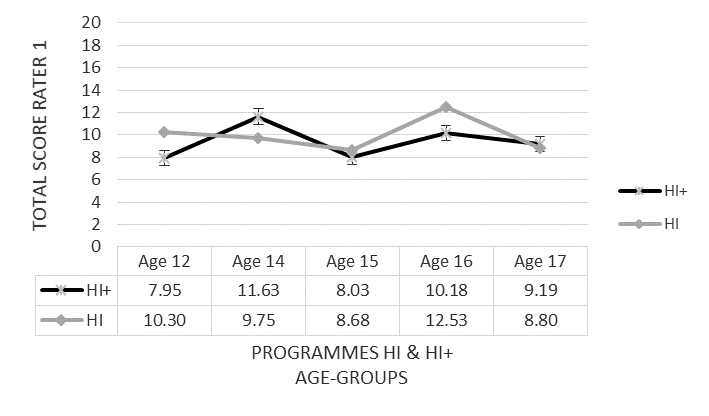
\includegraphics[width=\textwidth]{figures/tejada-img2.png}
% 
  \begin{tikzpicture}
    \begin{axis}[
	xlabel={Programmes HI \& HI+ Age-Groups},  
	ylabel={Total score rater 1}, 
	axis lines*=left, 
        width  = .8\textwidth,
	height = .45\textheight,
    	nodes near coords, 
	xtick=data,
	x tick label style={},  
	ymin=5,
	ymax=15, 
	symbolic x coords={Age 12, Age 14, Age 15, Age 16, Age 17},
	legend style={at={(1,0.4)},anchor=west}, 
	] 
	\addplot[draw=lsDarkBlue,thick] 
	    coordinates {(Age 12,7.95) (Age 14,11.63) (Age 15,8.03) (Age 16,10.08) (Age 17,9.19)};
	\addplot[draw=lsMidGreen,thick, dashed] 
	    coordinates {(Age 12,10.30) (Age 14,9.75) (Age 15,8.68) (Age 16,12.53) (Age 17,8.80)};
	\legend{HI, HI+}
    \end{axis} 
  \end{tikzpicture} 
 
 
% 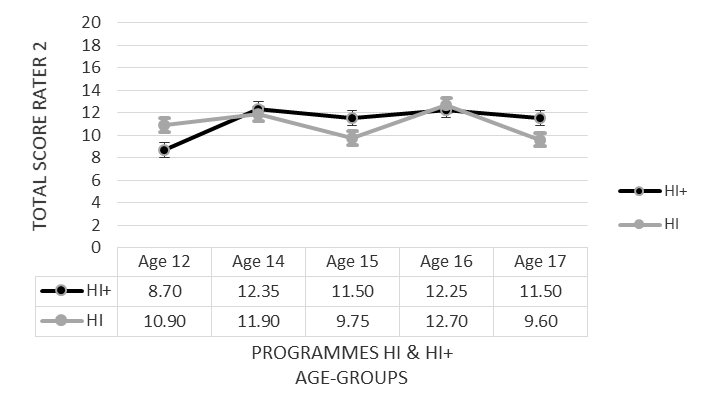
\includegraphics[width=\textwidth]{figures/tejada-img3.png}
  \begin{tikzpicture}
    \begin{axis}[
	xlabel={Programmes HI \& HI+ Age-Groups},  
	ylabel={Total score rater 2}, 
	axis lines*=left, 
        width  = .8\textwidth,
	height = .45\textheight,
    	nodes near coords, 
	xtick=data,
	x tick label style={},  
	ymin=5,
	ymax=15, 
	symbolic x coords={Age 12, Age 14, Age 15, Age 16, Age 17},
	legend style={at={(1,0.4)},anchor=west}
	] 
	\addplot[draw=lsDarkBlue,thick] 
	    coordinates {(Age 12,8.70) (Age 14,12.35) (Age 15,11.50) (Age 16,12.25) (Age 17,11.50)};
	\addplot[draw=lsMidGreen,thick, dashed] 
	    coordinates {(Age 12,10.90) (Age 14,11.90) (Age 15,9.75) (Age 16,12.70) (Age 17,9.60)};
	\legend{HI, HI+}
    \end{axis} 
  \end{tikzpicture} 
 
\end{figure}


Between-group comparisons using Welch’s t-test did not reveal any statistical differences between the programmes, as shown in \tabref{tab:tejada:8}. The mean difference between raters’ perception of HI+ and HI on various aspects of writing ability ranges from -0.17 to 0.03. These results suggest that neither programme is perceived as significantly different from the other, when it comes to the holistic rating of \isi{L2} \isi{writing performance}. 

\begin{table}
\footnotesize
\begin{tabularx}{\textwidth}{Q rrr rrrr}
\lsptoprule
&\raggedright \rotatehead[2cm]{\mbox{\bfseries Group HI+}\\ \bfseries  Mean (SD)}\hspace*{1cm} & 
 \raggedright \rotatehead{\mbox{\bfseries Group HI} \bfseries Mean~(SD)}\hspace*{1cm} & 
 \raggedright \rotatehead{\mbox{\bfseries Mean difference} \mbox{\bfseries between groups}}\hspace*{5mm} & 
  \bfseries \textit{t} & 
  \bfseries \textit{p} & 
  \bfseries 95\% CI & 
  \bfseries \textit{d}\\
\midrule
 Task fulfillment &\raggedleft 2.895 (0.69) & 2.928 (0.93) & {-0.033} & 0.191 & 0.84 & -0.293 0.355 & {0.03}\\
\tablevspace
 Text organisation&\raggedleft 2.355 (0.51) & 2.525 (0.82) & {-0.170} & 1.15 & 0.253 & {-0.112  0.422} & {0.23}\\
\tablevspace
{ Grammar}        &\raggedleft {2.615 (0.60)} & {2.628 (0.74)} & {-0.012} & {0.008} & {0.992} & {-0.264  0.266} & {0.001}\\
\tablevspace
 Vocabulary       &\raggedleft {2.530 (0.64)} & {2.50 (0.74)} & {0.030} & {-0.334} & {0.738} & -0.317  0.225 & -0.06\\
\tablevspace
 Total score      &\raggedleft 10.395 (2.17) & 10.520 (2.97) & {-0.125} & 0.161 & {0.871} & {-0.939 1.106} & {0.03}\\
\lspbottomrule
\end{tabularx}
\caption{\label{tab:tejada:8}: Analysis of between-group differences in holistic ratings by two evaluators (Welch’s T-Test)} 
\end{table}

\section{Discussion and conclusions}

This study has sought to understand whether the differential accumulated time of EFL-exposure (expressed in number of hours of \isi{L2} learning) has an impact on \isi{writing performance} in two \isi{immersion} programmes,  HI+ and  HI. They are different in the accumulated number of hours at all points throughout the programme, and clearly at the end, at learners’ 17 years of age, when the HI+ programme has accumulated 8,760  hours, while the HI programme 7,002. 

\isi{CAF} measures and holistic ratings of writing samples were scrutinised with a cross-sectional design in which learners were measured throughout the programme, on a yearly basis, starting at age 12. Concerning \isi{CAF}, four measures out of nine (IndepCS, CoordCR, \isi{DepCS}, Guiraud, D, TotalErr/100, GrErr/100, WS, WM) were found to be statistically different between programmes but not all in favour of HI+.  As regards complexity, IndepCS and \isi{DepCS}  were significantly lower for the HI+ group;  for accuracy, GrErr/100 were statistically higher for the HI+ group;  for \isi{fluency}, WS, again, was statistically lower for the HI+ group. In terms of \isi{lexical complexity} and the holistic ratings, no significant differences were found between the two programmes. 

Overall, it would seem to be the case that the two programmes are not substantially different in terms of learners’ outcomes in \isi{EFL} written performance. However, it cannot be said that they are entirely the same either. Indeed, the HI+ programme reveals lower levels in the domains of \isi{syntactic complexity} and \isi{fluency}, but higher levels for accuracy, and equal levels for \isi{lexical complexity}.  This has been also found in studies on the effects of a \isi{CLIL} course in \ili{English} added to \isi{conventional formal instruction} contrasted with a group only taking \isi{formal instruction}, as the latter outperformed the former, although not significantly (\citealt{RoquetPérez-Vidal2015}). 

Consequently, given its mixed results, this study partly questions the early assertions made by \citet{Carroll1962} and \citet{Stern1985} in the direction that more L2-exposure time would directly lead to more skilled language use. Our approach to the interpretation of these findings is in terms of time distribution of each of the two programmes, between learners’ ages 12 and 17, as presented in \tabref{tab:tejada:2} and \figref{fig:tejada:1}. In the case of HI+, learners undergo a decrease of L2-exposure time which goes from 672 hours a year to 612, and then to 480 (see \figref{fig:tejada:1}). This is not the case for HI pupils, who  receive fewer hours of target \isi{language exposure} per year, 504, yet at a steady rhythm. Additionally, the reduction in exposure is placed one year earlier for the HI+ group, that is at age 15,  than for the HI group, at age 16.

 On the one hand, such a contrast in the distribution of \isi{L2} exposure time in the two programmes allows us to suggest that gradual exposure to the \isi{L2} (HI programme) might explain the similarity in results with HI+, with more accumulated amount of \isi{L2} exposure yet less consistent in its distribution.

However, such a constant exposure experienced by the HI learners may also have had a less positive consequence; that is, the HI learners’ relative lower scores in terms of \isi{grammatical} accuracy. In this sense, the notion of \textit{stabilisation}, or \textit{plateauing}, proposed by \citet{Long2008} might be relevant. Indeed, a closer analysis of the learners’ performance suggests a plateau effect mainly concerning \isi{grammatical} accuracy, in the case of the HI programme predominantly observed in conjugation and agreement errors, a finding which has already been identified in \isi{immersion} learners in the literature (\citealt{Rifkin2005,HartEtAl1991}). HI’s outcomes in accuracy could be interpreted as a level of ``maintenance'' achieved in this programme. These findings can be relative to the regular and steady amount of exposure for HI students in primary and between ages 12 and 15 in secondary school, as exposed in \figref{fig:tejada:1}.

On this note, \citegen{Bournot-Trites2007} findings are only partially confirmed in our case. In her study, no significant differences in writing quality were found between two groups of secondary \isi{immersion} students with different L2-French intensity. In addition, \citegen{Bournot-Trites2007} study reveals a plateau effect in the field of grammar accuracy (particularly tense markers) and lexical diversity, where she observes: ``it seems that after a certain threshold of competence in [\isi{L2}], the increase in the time spent in this language in the class does not improve much the quality of the written production of pupils'' \citep[20]{Bournot-Trites2007}.  

Likewise, the similarity of the two programmes in terms of \isi{lexical complexity} could also be explained in terms of input exposure. It would seem that neither programme offers complementary hours of exposure outside of the classroom which would aid learners to make progress in such a domain. 

Concerning the lower levels of \isi{fluency} found in the HI+ group, they could be attributed either to the programme’s didactic approach, or to task effects which remain to be explored in future research.  

Some limitations of this study need to be acknowledged. First the unbalance in the sample size where the HI+ programme includes a larger number of subjects than HI, which is represented by fewer subjects. Second, task conditions as well as task variety (in terms of complexity and text genres) need to be reconsidered. Further research might include different types of tasks and writing genres with different cognitive demands. We should additionally underscore that the HI programme-related positive results, which refer to denser, richer texts, may be associated to the emphasis on literacy in the HI’s curriculum described in section 4.1.1. The task might have been more familiar to HI students and therefore yielded to slightly more syntactically complex and organised texts. 

To conclude, the present study has confirmed that the examination of the time factor in L2-\isi{acquisition} in formal educational settings remains a rather complex endeavour due to a number of methodological constraints and issues. It is difficult to assess different programmes at exactly the same times (in terms of age, \isi{L2} exposure, curriculum years), and to control for programme features.  Future research is needed to pursue research in bilingual schools or \isi{immersion} programmes in non-\ili{English} speaking contexts and to explore performance differences among different age groups, with a mixed methods approach including the holistic analyses suggested.

\section*{Acknowledgments}

The authors are grateful to the anonymous reviewer as well as to Gabriele Pallotti for their insightful comments and contributions to this chapter. Also we would like to thank Cylcia Bolibaugh for her statistical advice. Isabel would like to thank Alejandra Plata and Alejandro Mejia from Uniandes for their help with earlier versions of this text.
 
\sloppy
\printbibliography[heading=subbibliography,notkeyword=this] 
\end{document}